\chapter{Stand der Technik}
\label{ch:StandDerTechnik}

Das erste \gls{RFID}-System wurde von den Allierten im Zweiten Weltkrieg eingesetzt. Deren Freund-Feind-Erkennung funktionierte über eine passive Reflektion der Radarwellen, welche auf die Frequenz der Radarsender geeicht war. Verbündete Flieger ergaben dadurch ein viel stärkeres Signal und waren als hellere Punkte erkennbar (\cite{chawla2007}, \cite{uswardep1946_3}). In den 1960er wurden in den USA verschiedenste Patente angemeldet, welche sich das Prinzip der elektromagnetischen Induktion zunutze machen, um sich gegenüber einem Sender zu identifizieren. Die Adaption der Technologie liess jedoch auf sich warten, \citeauthor{want2004} identifiziert als Grund dafür die fehlende Marktviabilität, die Ausgereiftheit der Technologie selbst und die Adaptionskosten \parencite{want2004}. All dies hat sich in den 60 Jahren seither geändert und \gls{RFID} ist eine etablierte Technologie, welche in verschiedensten Bereichen eingesetzt wird.

\section{Technologische Grundlagen}

Ein \gls{RFID} System besteht generell aus zwei Teilen: Einem Sender und Empfänger, diese werden Interrogator (dt. Anfragender) und Transponder (dt. Sendegerät) genannt. Der Transponder wird auch als \gls{RFID} Tag bezeichnet und kann sowohl passiv, das heisst ohne Stromversorgung auf dem Tag, wie auch aktiv sein, das heisst der Chip und die Antenne werden durch eine integrierte Batterie versorgt. Der Vorteil eines aktiven Tags liegt in dessen höherer Reichweite. Als Mischung zwischen den Beiden ist der semi-aktive Tag, bei dem nur der Chip durch die Batterie mit Energie versorgt wird, und die Antenne durch das Feld des Interrogators gespiesen wird.

Bei der Funktionsweise von \gls{RFID} Tags muss man zwischen zwei Funktionalitäten unterscheiden, welche auf die Entfernung zwischen Transponder und Interrogator abhängig sind. Im Nahbereich (engl. Near-Field \gls{RFID}) funktioniert die Stromversorgung über magnetische Induktion, wobei die Arbeitsspannung der Chips im Mikro- bis Miliwattbereich liegt. Die Kommunikation zwischen Interrogator und Transponder wird über "load modulation"\ realisiert. Dies bedeutet, dass der Transponder, aktiviert durch das Feld des Interrogator, selber beginnt ein Feld auszustrahlen. Dadurch entstehen Interferenzen im Feld, welche sich durch minimale Spannungsänderungen in der Spule des Interrogators messen lassen \parencite{want2006}. Die Distanz des Nahfelds ist durch die Gleichung \ref{NearFieldEM} gegeben. Für \gls{HF} Tags (wie diejenigen die auch in der Speicherbibliothek verwendet werden) ist die Betriebsfrequenz durch den ISO Standard 18000-3 auf 13.56MHz festgelegt und ergibt damit eine theoretisch maximale Distanz von 3.519m für das Nahfeld. Im realen Umfeld mit dem ISO 18000-3 Standard, welcher die Sendeleistung des Interrogator auf 12A/m beschränkt, beträgt die maximale Distanz circa einen Meter \parencite{ISO18000-3}.

\indexequation{d=\frac{\lambda}{2\pi}}{Reichweite des reaktiven Nahfelds}{NearFieldDistance}
\indexequation{\lambda=\frac{c}{f}}{Definition der Wellenlänge $\lambda$ in Abhängigkeit der Lichtgeschwindigkeit c}{Wavelength}
\indexequation{d=\frac{c}{2\lambda\pi}}{Definition der Wellenlänge in Gleichung \ref{NearFieldDistance} eingesetzt}{NearFieldEM}

Im Fernfeldbereich erhält der \gls{RFID} Tag die Energie direkt über die ausgestrahlte Elektromagnetischen Wellen. Die Abnahme der Energiedichte auf Distanz ist dabei proportional zu $\frac{1}{r^2}$. Dennoch ist es, durch Fortschritte in der Miniaturisierung und besserer Energieeffizienz moderner Halbleiter und Chips, möglich geworden dadurch \gls{UHF} Tags mit Strom zu versorgen. 
Die Kommunikation funktioniert mittels "back scattering"\, dabei absorbiert eine Antenne, welche auf eine bestimmte Frequenz eingestellt ist, den Grossteil der Wellen die gesendet werden. Passt jedoch die Impedanz nicht genau, so reflektiert die Antenne ein Teil des Signals an die Quelle, den Interrogator, zurück. Die Anpassung der Impedanz der Antenne, über die Zeit, führt dazu, dass mehr oder weniger des Signales reflektiert wird, womit eine Nachricht codiert übermittelt werden kann \parencite{want2006}.


\begin{figure}[htb]
	\centering
	\begin{subfigure}[b]{0.8\linewidth}
		\centering
		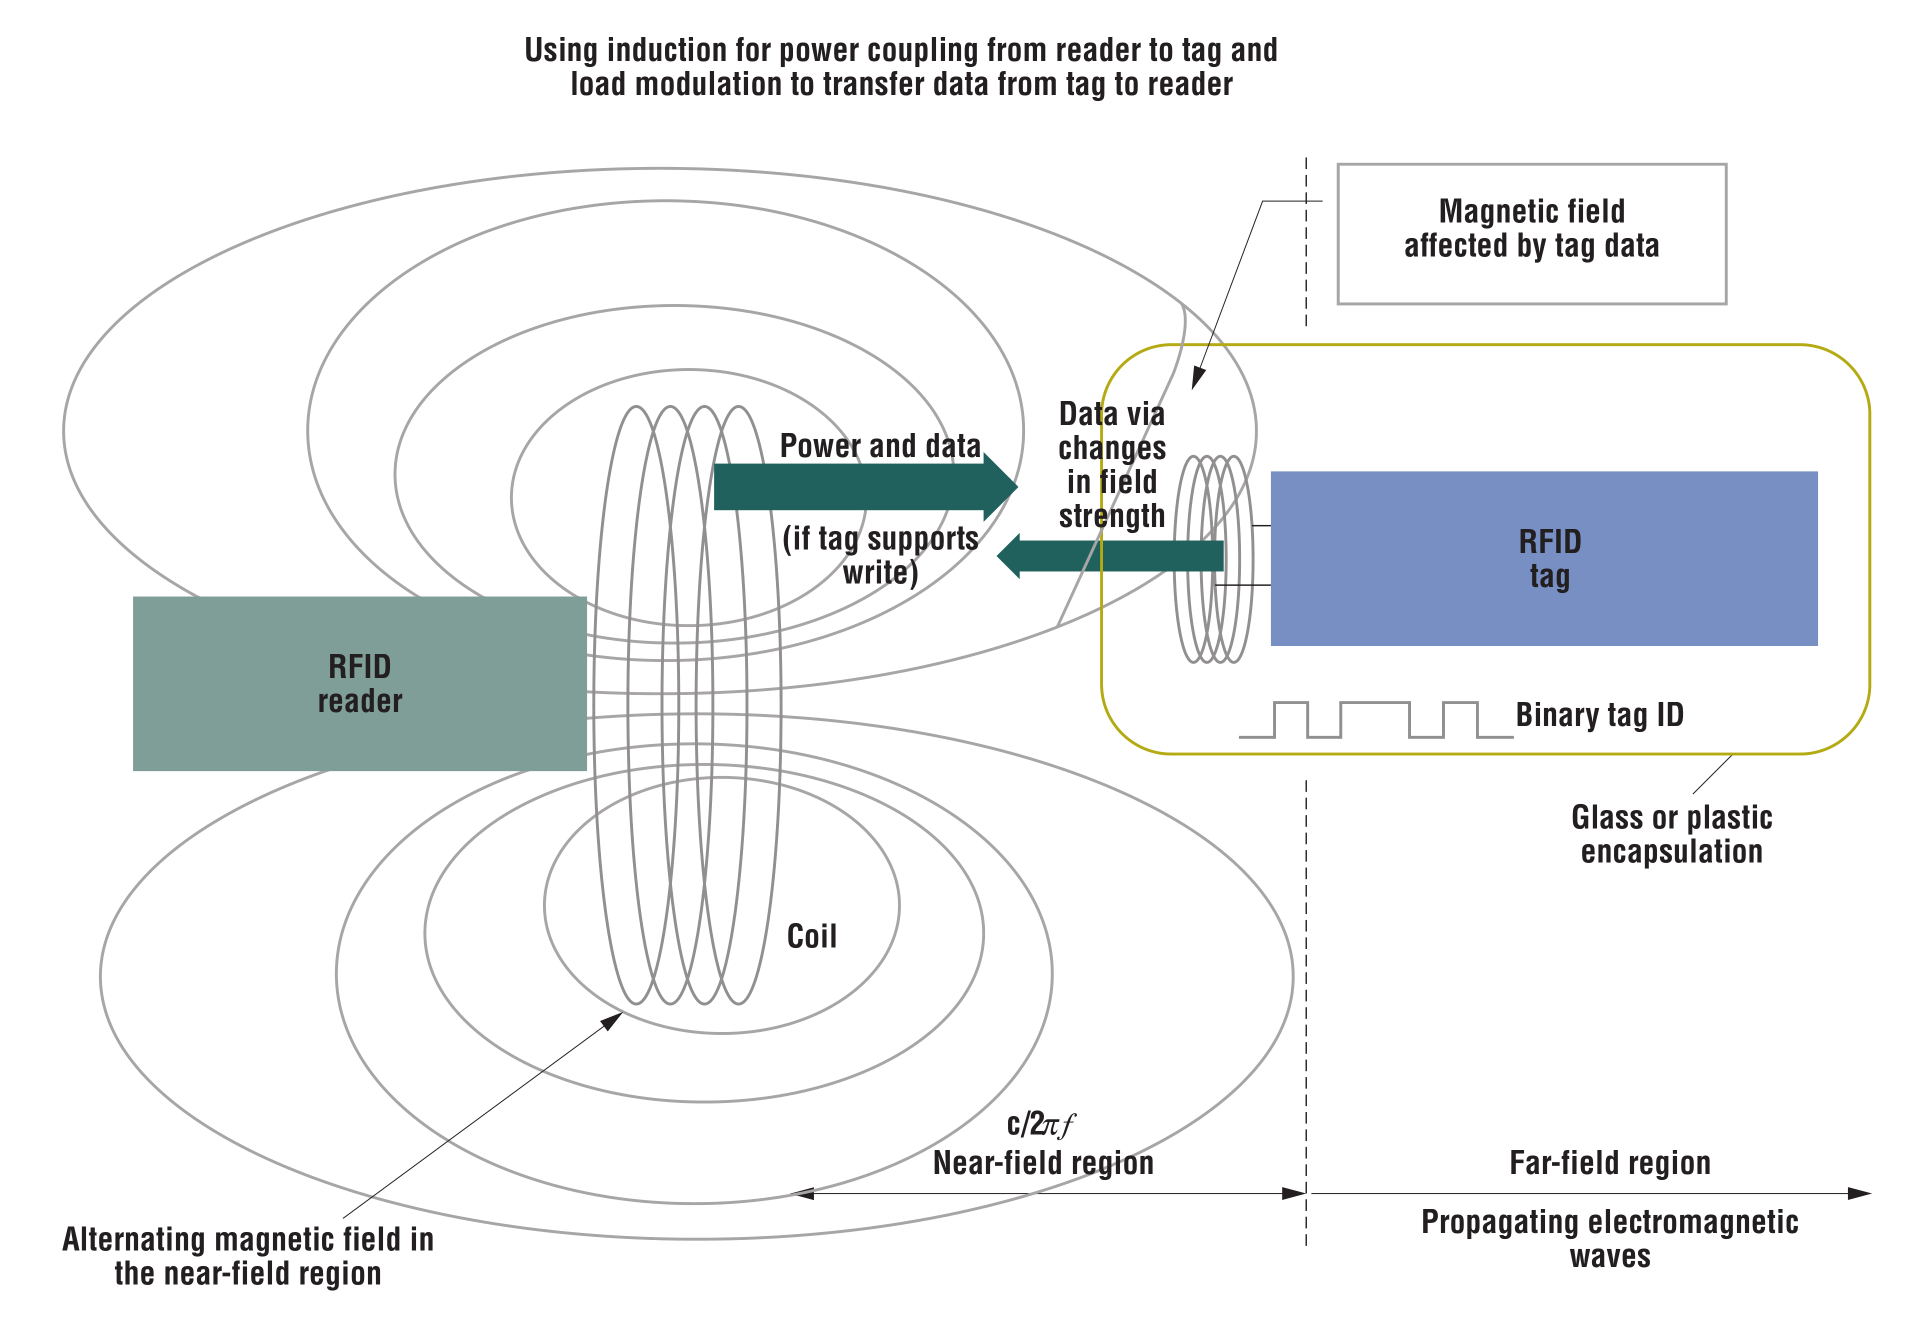
\includegraphics[keepaspectratio,width=\linewidth]{InductionCoupling}
		\caption{Magnetische Induktion und "load modulation"}
	\end{subfigure}
	\begin{subfigure}[b]{0.8\linewidth}
		\centering
		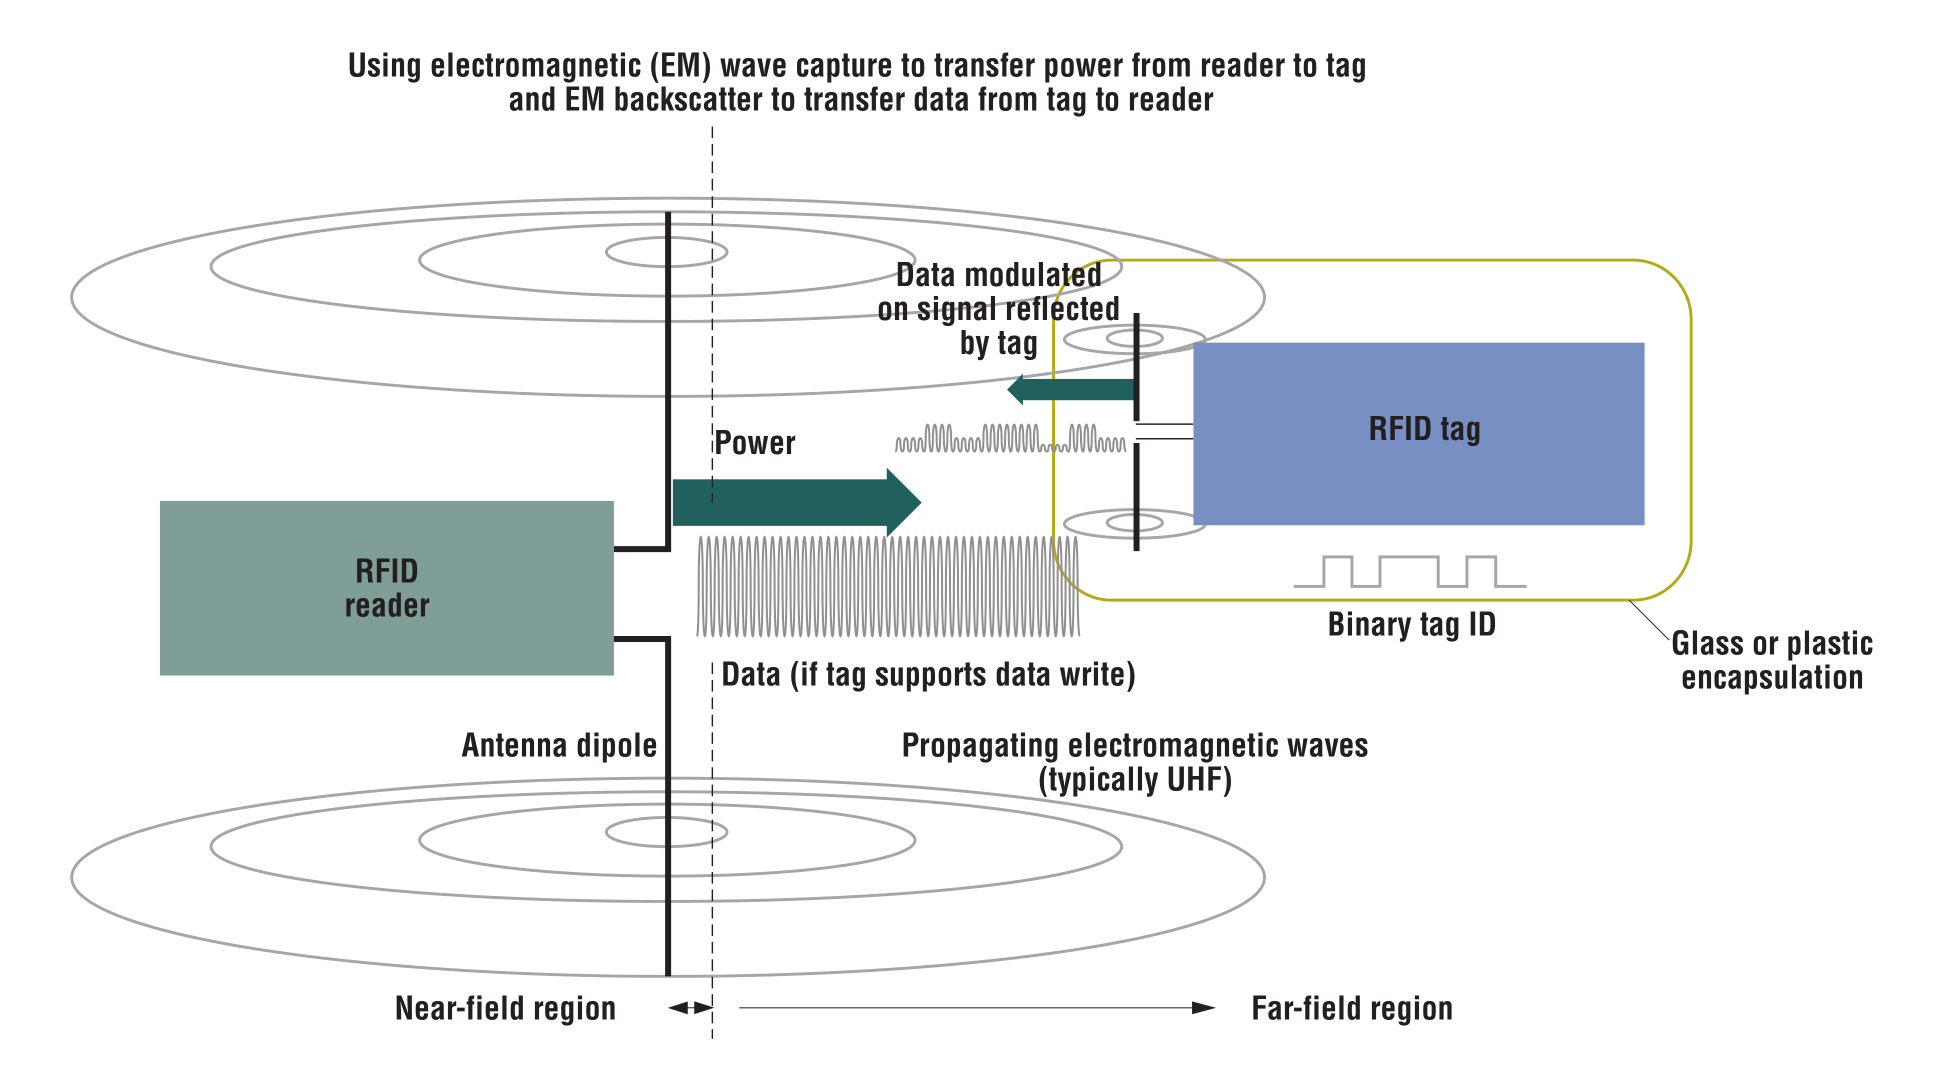
\includegraphics[keepaspectratio,width=\linewidth]{Backscattering}
		\caption{EM Wellentransmission und "backscattering"}
	\end{subfigure}
	\caption{Funktionsweisen von Nah- und Fernfeld \gls{RFID} Tags graphisch dargestellt \parencite{want2006}}
\end{figure}

\section{Technische Konzepte}

Da auf eine Anfrage eines Interrogators alle Chips in dessen Nähe antworten, ist der Luft\-raum daher als eine Kollisionsdomäne zu verstehen. Dies bedeutet, dass alle beteiligten Parteien auf dem gleichen Medium sind, sich also gegenseitig stören können. Dieses Problem kennt man in der Netzwerktechnik seit Tokenring, und heutzutage vor allem im WLAN Bereich. Die bei \gls{RFID} verwendete Strategie ist dabei die Kollisionsvermeidung und funktioniert nach dem folgenden Prinzip:
\begin{enumerate}
	\item Ein Tag sendet nur nach Empfang der kompletten Befehlssequenz des Interrogator
	\item Ein Tag sendet nur falls er spezifisch angefragt wurde
\end{enumerate}
Der Interrogator unterteilt daher während einer Inventur seine Anfrage in unterschiedliche Zeitbereiche. Pro Bereich fragt er nach den Identifikationsnummern von Tags mit einer Maske, diese Antworten nur falls die Maske auf Ihre Identifikationsnummer passt. Geschieht dabei eine Kollision, so wird der betreffende Bereich weiter unterteilt, bis das ganze Inventar erfasst wurde \parencite{ISO15693-3}.

Für \gls{RFID} sind in den ISO Diskussionen verschiedene Frequenzen festgelegt worden. Diese bieten unterschiedliche Vor- und Nachteile welche in der Tabelle \ref{tbl:RFIDFrequencies} dargestellt werden.

\begin{table}[htb]
	\begin{tabularx}{\textwidth}{|X|X|X|X|X|}
		\hline
		\textbf{Frequenz\-bereich} & \textbf{LF (< 135kHz)} & \textbf{HF (13.56MHz)} & \textbf{UHF (860-960MHz)} & \textbf{Mikrowelle (2.45GHz)}\\
		\hline
		\textbf{Lesereichweite} & <0.5m & \textasciitilde 1m & \textasciitilde 4-5m & \textasciitilde 1m\\
		\hline
		\textbf{Typ} & passiv & passiv & passiv oder aktiv & passiv oder aktiv\\
		\hline
		\textbf{Parallele Leserate} & langsam & langsam & schnell & schnell \\
		\hline
		\textbf{Interferenz durch Wasser und Metal} & wenig & wenig & viel & viel \\
		\hline
		\textbf{Grösse der Tags} & gross & gross & klein & klein \\
		\hline
	\end{tabularx}
	\caption{Vor- und Nachteile der unterschiedlichen Betriebsfrequenzen von \gls{RFID} Tags \parencite{chawla2007}}
	\label{tbl:RFIDFrequencies}
\end{table}
